\section{Задание}

В информационный центр приходят клиенты через интервал времени $10\pm2$  минуты.
Если все три имеющихся оператора заняты, клиенту отказывают в обслуживании.
Операторы имеют разную производительность и могут обеспечивать обслуживание среднего запроса пользователя за $20\pm5$; $40\pm10$; $40\pm20$.
Клиенты стремятся занять свободного оператора с максимальной производительностью.
Полученные запросы сдаются в накопитель. Откуда выбираются на обработку.
На первый компьютер запросы от 1 и 2-ого операторов, на второй -- запросы от 3-его.
Время обработки запросов первым и 2-м компьютером равны соответственно 15 и 30 мин.
Промоделировать процесс обработки 300 запросов. 

\section{Теоритическая часть}

Необходимо создать концептуальную модель в терминах СМО, определить эндогенные и экзогенные переменные и уравнения модели.
За единицу системного времени выбрать 0,01 минуты.

\begin{figure}[h!]
\centering
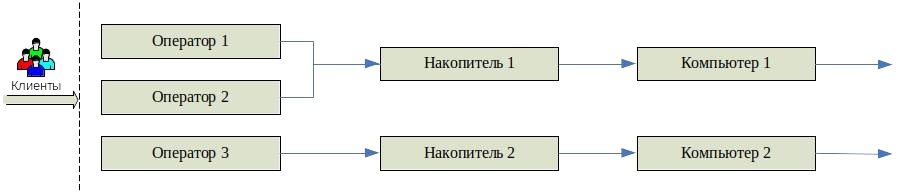
\includegraphics[width=\textwidth]{5/5_1}
\end{figure}


В процессе взаимодействия клиентов с информационным центром возможно:

\begin{itemize}
    \item Режим нормального обслуживания, т.е. клиент выбирает одного из свободных операторов, отдавая предпочтение тому у которого меньше номер.
    \item Режим отказа в обслуживании клиента, когда все операторы заняты
\end{itemize}

Переменные и уравнения имитационной модели.

\begin{itemize}
    \item Эндогенные переменные: время обработки задания i-ым оператором, время решения этого задания j-ым компьютером.
    \item Экзогенные переменные: число обслуженных клиентов и число клиентов получивших отказ.
\end{itemize}



\begin{figure}[h!]
\centering
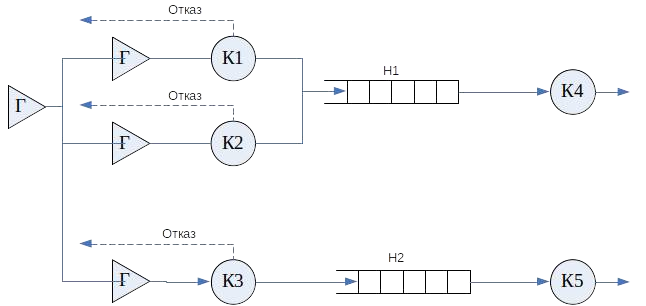
\includegraphics[width=0.82\textwidth]{5/5_2}
\end{figure}

Вероятность отказа:
\begin{equation*}
    P_{\text{отк}} = \frac{C_{\text{отк}}}{C_{\text{отк}} + C_{\text{обсл}}}
\end{equation*}

\pagebreak
\vbox{}
\section{Результаты}

\lstinputlisting[basicstyle=\fontsize{9}{10}\ttfamily]{7/result.txt}

\pagebreak
\section{Листинг кода}

\lstdefinelanguage{GPSS}{
	keywords={GENERATE, GATE, NU, SEIZE, ADVANCE, RELEASE, TRANSFER, QUEUE, DEPART, SAVEVALUE, TERMINATE},
	keywordstyle=\color{blue}\bfseries,
	ndkeywords={START},
	ndkeywordstyle=\color{purple}\bfseries,
	identifierstyle=\color{black},
	sensitive=false,
	comment=[l]{;}
}

\lstinputlisting[language=GPSS,basicstyle=\fontsize{9}{10}\ttfamily]{../7/main.txt}